\chapter{IPv4 Addressing: Part 2}\label{ipv4-addressing-part-2}

\section{Maximum Hosts per Network}\label{maximum-hosts-per-network}

Let's take a Class C Network:

192.168.1.0/24

(gives a range of 0 ---\textgreater{} 255)

Said another way, the HOST portion (the .0) is equal to 8 bits
so\ldots{}

Host portion = 8 bits = 2\^{}8 = 256

HOWEVER, since the Network Address (Network ID)

192.168.1.0 is Reserved

AND

192.168.1.255 (BROADCAST ADDRESS) is ALSO reserved.

The MAXIMUM Hosts per Network = 2\^{}8-2 = 254 hosts

What about a Class B Network ?

172.16.0.0/16 ----\textgreater{} 172.16.255.255/16

Host portion = 16 bits = 2\^{}16 = 65,536

Maximum hosts per network = 2\^{}16-2 = 65,534 hosts

What about a Class A Network ?

10.0.0.0/8 -------------\textgreater{} 10.255.255.255/8

Host portion = 24 bits = 2\^{}24 = 16,777,216

Maximum hosts per network = 2\^{}24-2 = 16,777,214 hosts

\section{Therefore}\label{therefore}

The formula for calculating the number of HOSTS on a network is:

2 \^{} N - 2 (2 to the power of N - 2)

where N = number of HOST bits

\section{First / Last Usable
Addresses}\label{first-last-usable-addresses}

Class C Network

192.168.1.0/24 (NETWORK ADDRESS)

Add 1 so the Host Portion = 00000001

192.168.1.1/24 = FIRST USABLE ADDRESS

192.168.1.255/24 (BROADCAST ADDRESS)

Subtract 1 from the BROADCAST ADDRESS = 11111110

192.168.1.254/24 = LAST USABLE ADDRESS

Class B Network

172.16.0.0/16 (NETWORK ADDRESS)

Add 1 to Host portion so 0000 0000 0000 0001

172.16.0.1/16 is the FIRST USABLE ADDRESS

172.16.255.255/16 (BROADCAST ADDRESS)

Subtract 1 to Broadcast Address so 1111 1111 1111 1110

172.16.255.254/16 is the LAST USABLE ADDRESS

Class A Network

10.0.0.0/8 (NETWORK ADDRESS)

Add 1 to Host portion so 00000000 00000000 00000001

10.0.0.1/8 is the FIRST USABLE ADDRESS

10.255.255.255/8 (BROADCAST ADDRESS)

Subtract 1 to Broadcast Address so 1111 1111 1111 1110

10.255.255.254/16 is the LAST USABLE ADDRESS

\section{Cisco CLI Device
Configuration}\label{cisco-cli-device-configuration}

R1\textgreater{} enable R1\# show ip interface brief

Lists the Interfaces, IP Addresses, Method, Status, and Protocol.

Interfaces:

\begin{itemize}
\tightlist
\item
  What port interfaces are available/connected
\end{itemize}

IP Addresses

\begin{itemize}
\tightlist
\item
  Self explanatory. What IP Address is assigned.
\end{itemize}

Method

\begin{itemize}
\tightlist
\item
  What method was the IP address assigned?
\end{itemize}

Status (Layer 1 Status)

\begin{itemize}
\tightlist
\item
  Current status of interface
\item
  `administratively down' = Interface has been disabled with the
  `shutdown' command
\end{itemize}

Administratively down is the DEFAULT status of Cisco Router interfaces.

Cisco Switch interfaces are NOT administratively down by DEFAULT.

Protocol (Layer 2 Status)

\begin{itemize}
\tightlist
\item
  Cannot operate if Status (Layer 1) is down
\end{itemize}

\begin{figure}
\centering
\pandocbounded{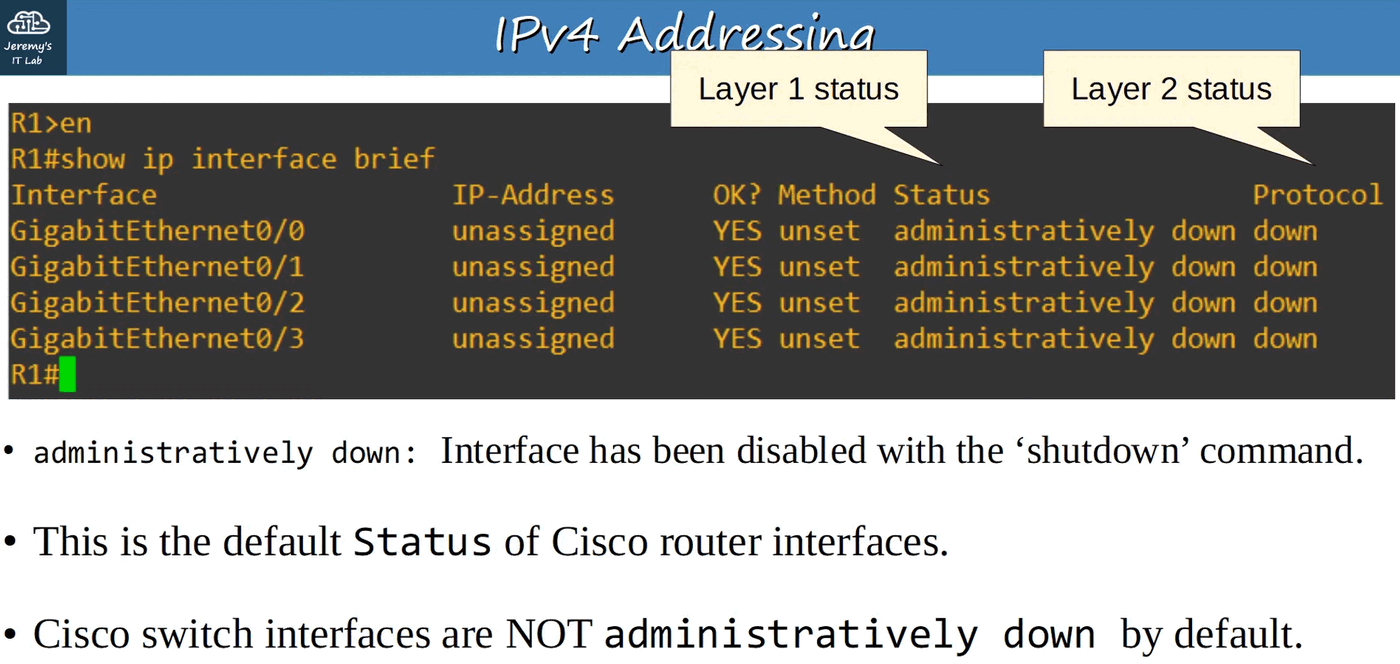
\includegraphics[keepaspectratio,alt={image}]{images/08-ipv4-addressing-part2/img-001.png}}
\end{figure}

// configure terminal cmd

R1\# conf t

// This enters interface configuration mode

R1(config)\# interface gigabitethernet 0/0

This can be shortened to `g0/0' like they are listed in physical network
maps.

\begin{figure}
\centering
\pandocbounded{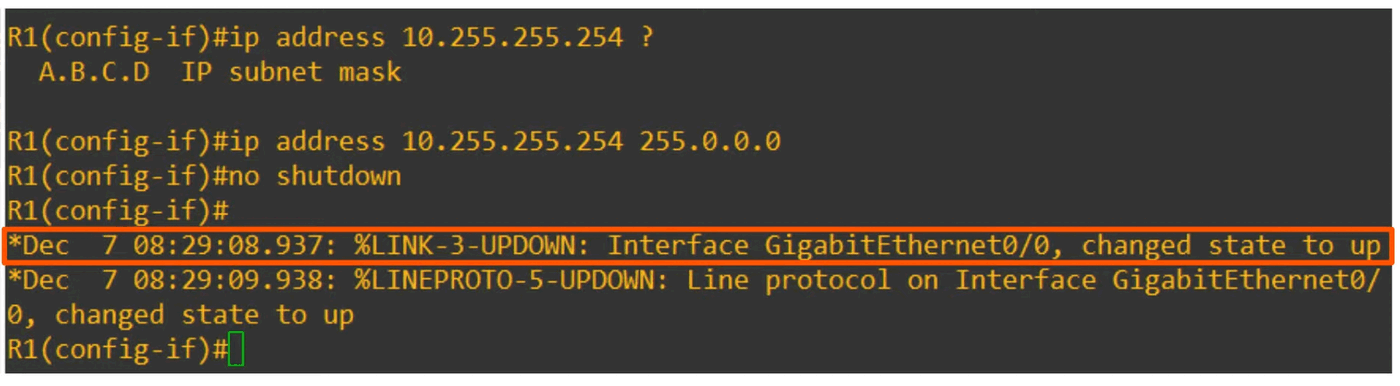
\includegraphics[keepaspectratio,alt={image}]{images/08-ipv4-addressing-part2/img-002.png}}
\end{figure}

// This sets the IP ADDRESS and SUBNET MASK of device

R1(config-if) \#ip address 10.255.255.254 255.0.0.0

// This enables the device

R1(config-if) \#no shutdown

Two messages should appear showing the state has changed to `up'
(Status). Second message should show line protocol is now `up'
(Protocol).

// `do' allows you to run a Privileged EXEC command from outside the
mode.

R1(config-if) \#do show ip interface brief

Good to confirm that the device/interface you have configured is up and
running.

More `show' CLI Commands

\begin{figure}
\centering
\pandocbounded{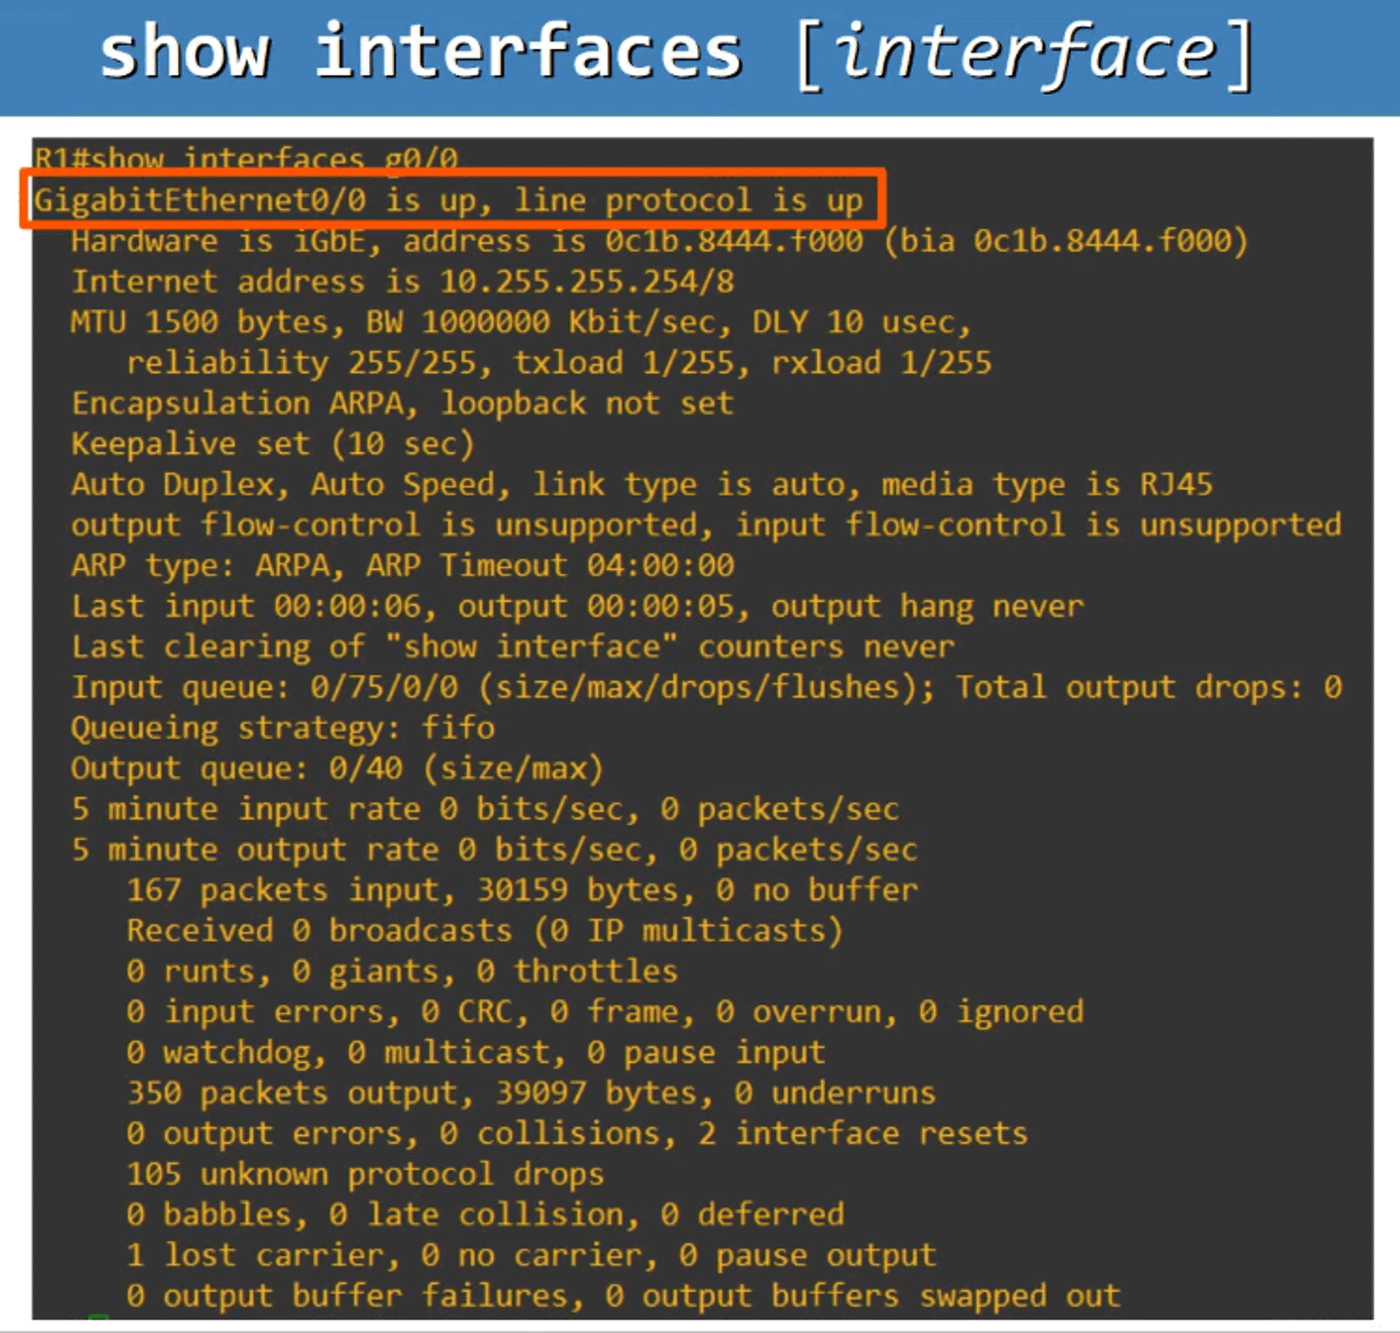
\includegraphics[keepaspectratio,alt={image}]{images/08-ipv4-addressing-part2/img-003.png}}
\end{figure}

`show interfaces \textless interface name\textgreater{}'

\begin{itemize}
\tightlist
\item
  Shows Layer 1 and Layer 2 information about the interface and some
  Layer 3.
\item
  Shows MAC Address (or BIA address)
\item
  IP Address
\item
  \ldots{} and so much more
\end{itemize}

`show interfaces description'

\begin{itemize}
\tightlist
\item
  show description for interface.
\end{itemize}

Example:

// Configure mode for interface Gigabyte Interface 0/0

R1(config) \#int g0/0

R1(config) \#description \#\# to SW1 \#\#

This sets the `Description' column to display:

\begin{lstlisting}
Interface               Description
\end{lstlisting}

Gi0/0 \#\# to SW1 \#\#
